\documentclass[aps,prd,twocolumn,superscriptaddress,nofootinbib,longbibliography]{revtex4-2}

\usepackage[utf8]{inputenc}
\usepackage[T1]{fontenc}
\usepackage{amsmath,amssymb,bm}
\usepackage{mathrsfs}
\usepackage{graphicx}
\usepackage{booktabs}
\usepackage{array}
\usepackage[colorlinks=true,linkcolor=blue,citecolor=blue,urlcolor=blue]{hyperref}

\newcommand{\dd}{\mathrm{d}}
\newcommand{\Lag}{\mathcal{L}}
\newcommand{\LD}{\mathfrak{L}}
\newcommand{\calS}{\mathcal{S}}
\newcommand{\calC}{\mathcal{C}}
\newcommand{\calD}{\mathcal{D}}
\newcommand{\Mp}{M_{\rm p}}
\newcommand{\Lam}{\Lambda}
\newcommand{\LCDM}{\Lambda{\rm CDM}}
\newcommand{\DES}{\mathrm{DES}}
\newcommand{\DESI}{\mathrm{DESI}}
\newcommand{\SN}{\mathrm{SN}}
\newcommand{\BAO}{\mathrm{BAO}}
\newcommand{\varphione}{\varphi_1}
\newcommand{\varphitwo}{\varphi_2}
\newcommand{\chiT}{\chi^2_{\rm tot}}
\newcommand{\Riemsq}{R_{\mu\nu\rho\sigma}R^{\mu\nu\rho\sigma}}

\begin{document}

\preprint{AI-MG-v5.2.2-agent}

\title{Dark Energy Autonomous Search from Cosmological Background Data}

\author{Cooper Niu}
\affiliation{Department of Physics, Brown University, Providence, Rhode Island 02912, USA}

\author{Wenrong Sun}
\affiliation{Department of Physics, Brown University, Providence, Rhode Island 02912, USA}

\date{\today}


\begin{abstract}
We present a physics-first autonomous search for two-scalar modified-gravity backgrounds and use it to benchmark several large-language-model proposal policies under an identical deterministic validation pipeline.  Candidate theories are generated as covariant, dimension-balanced Lagrangian densities built from curvature tensors, covariant derivatives, and two scalar fields.  They are then subjected to symbolic FLRW equation-of-motion filtering, algebraic cancellation of independent third- and higher-time derivatives, Builder conversion into numerical models, and direct comparison with DES type-Ia supernovae and DESI Data Release 2 baryon-acoustic-oscillation distances.  The artificial-intelligence component affects only the proposal distribution over legal operator combinations and explicit parameter samples; ghost filtering, numerical regularity, constraint preservation, and the final ranking by $\chi^2_{\rm tot}$ are determined by the physics code.  We report matched cold-start benchmark runs with 600 initial theory attempts for five proposal models: GPT-5.5, Claude Opus 4.8, Gemini 3.1 Pro, Qwen 3.7 Plus, and DeepSeek V4 Pro.  The fixed $\Lambda$CDM reference gives $\chi^2_{\rm tot}=1645.28$.  All agents find Einstein--Hilbert-anchored scalar backgrounds with $\chi^2_{\rm tot}\simeq 1638$, improving the reference by $\Delta\chi^2\simeq 7.1$--$7.3$.  DeepSeek V4 Pro obtains the lowest open-search value, $\chi^2_{\rm tot}=1637.953$, and the most concentrated set of high-quality open-search hits, but is the slowest proposal policy.  Claude Opus 4.8 and GPT-5.5 are the most efficient in wall-clock attempts per hour while remaining competitive.  Qwen 3.7 Plus is less stable in the open-search sector but produces the largest number of non-Einstein--Hilbert hits below $\chi^2_{\rm tot}=2000$.  The non-EH sector repeatedly converges to a cutoff-normalized $\phi_2$ curvature-squared branch near $\chi^2_{\rm tot}=1946.87$, which is substantially better than the generic failed plateau but not competitive with EH-anchored backgrounds.  These results benchmark proposal policies for background discovery; they do not by themselves establish full covariant ghost freedom, perturbation stability, structure-growth viability, gravitational-wave consistency, or local-gravity screening.
\end{abstract}

\maketitle


\section{Introduction}
\label{sec:introduction}

The observed acceleration of the Universe is one of the clearest indications that either the cosmic energy budget or the gravitational sector is not yet fully understood.  The minimal $\Lambda$CDM model gives a compact effective description of current background data, but it treats the late-time vacuum-energy scale as an input and does not explain whether the acceleration is produced by a rigid cosmological constant, additional fields, or modified gravitational dynamics.  Scalar-tensor and higher-curvature theories offer a controlled language for testing this possibility, but they also create a search problem: once curvature invariants, covariant derivatives, and multiple scalar fields are allowed, the space of covariant Lagrangians is far too large to inspect manually \cite{Clifton2012,SotiriouFaraoni2010,Horndeski1974}.

Most points in this large theory space are not physically acceptable.  Generic higher-derivative theories contain Ostrogradsky modes \cite{Ostrogradsky1850}; many proposed covariant densities do not admit a regular FLRW initial-value problem; many numerically regular branches violate the modified Friedmann constraint during integration; and most surviving backgrounds fit DES supernova and DESI BAO distances poorly.  A useful autonomous search must therefore be physics-first: an agent may propose structures, but deterministic symbolic and numerical code must decide whether the proposal is legal, stable at the background-filter level, numerically solvable, and empirically competitive.

The framework used here follows this division of labor.  A proposal model chooses a scalar configuration, a grammar-constrained set of covariant operators, and an explicit list of parameter samples.  The proposal is then compiled into an isolated Lagrangian and passed through the same pipeline for every agent: symbolic FLRW variation, equation-level cancellation of independent third- and higher-time derivatives, Builder construction of a dimensionless initial-value problem, Solver integration, modified Friedmann-constraint monitoring, and comparison with DES-SN and DESI-DR2 BAO data \cite{DES2024SN,DESI2025BAO}.  The AI system does not estimate $\chi^2$, bypass the grammar, or override a failed physics stage.  This design is close in spirit to formal-language approaches to autonomous theory discovery, but the grammar and validation stages are those of modified gravity rather than particle interactions \cite{Alexander2026Albert}.

The present paper has two goals.  First, it summarizes the covariant theory space, FLRW derivative-order filter, constraint logic, dimensionless cosmological system, and sampling prescription used in the current code base.  These ingredients define what is meant by an accepted background branch.  Second, it reports a matched five-model benchmark of the proposal layer.  We compare GPT-5.5, Claude Opus 4.8, Gemini 3.1 Pro, Qwen 3.7 Plus, and DeepSeek V4 Pro on the same cold-start task, with two discovery sectors: an open-search sector that may include the Einstein--Hilbert anchor, and a non-EH sector that forbids the bare $R$ term and searches for new-physics backgrounds without explicit EH support.  The comparison is organized around global optimum quality, new-physics discovery, speed/efficiency, robustness/stability, and acceptance rate.

The results should be interpreted with care.  The background data strongly favor EH-anchored scalar histories, and many low-$\chi^2$ operator lists are nearly degenerate with simple EH plus scalar baselines on FLRW.  Conversely, the non-EH sector repeatedly finds a recognizable $\phi_2$ curvature-coupled branch near $\chi^2_{\rm tot}\simeq 1946.87$, but this branch is not competitive with the open-search optimum.  These outcomes are useful: they identify where the current grammar and priors easily reproduce high-quality expansion histories, where genuinely non-EH searches remain difficult, and how different proposal models trade exploitation, exploration, and wall-clock speed.  They are not final claims of full theory viability; perturbation stability, structure growth, gravitational waves, local tests, and a more complete operator-redundancy audit remain separate validation layers.

\section{Covariant Theory Space}
\label{sec:theory-space}

\subsection{Dimension-balanced effective Lagrangians}
\label{subsec:dimension-balanced}

We consider a broad EFT-like space of metric theories containing two scalar fields, $\phi_1$ and $\phi_2$, with different characteristic scales.  A generated theory is stored and validated as a Lagrangian density,
\begin{equation}
\calS=\int \dd^4x\,\mathscr{L},
\qquad
\mathscr{L}=\sqrt{-g}\,\Lag ,
\label{eq:action}
\end{equation}
with the scalar bracket
\begin{equation}
\Lag=
\Mp^2\sum_{I\in G\cup N}
c_I\Lam^{2-d_I}O_I
+
\sum_{J\in S}c_J\Lam^{4-d_J}S_J
+
\Lag_{\rm fixed}.
\label{eq:lagrangian}
\end{equation}
Here $G$ denotes pure-curvature invariants, $N$ non-minimal scalar-curvature invariants, and $S$ pure-scalar generated invariants.  The integer $d_I$ is the mass dimension of the corresponding covariant scalar.  The factors of $\Mp^2$ and $\Lam$ ensure that each term in the density $\mathscr{L}$ has the correct mass dimension.  Thus a candidate is not specified by an operator label alone; its sector, coefficient, cutoff power, Planck-mass prefactor, fixed scalar matter terms, and outer $\sqrt{-g}$ are part of the physical theory.

The candidate building blocks include
\begin{equation}
R,\qquad R_{\mu\nu},\qquad R^\rho{}_{\sigma\mu\nu},\qquad
\nabla_\mu,\qquad \phi_1,\qquad \phi_2 .
\end{equation}
Examples of generated invariants are
\begin{equation}
R^2,\qquad
R_{\mu\nu}R^{\mu\nu},\qquad
\phi_1^2R,\qquad
\nabla_\mu\phi_1\nabla_\nu\phi_1R^{\mu\nu},\qquad
\Box\phi_1\,R.
\end{equation}
Up to mass dimension six, there are 141 independent curvature invariants on the FLRW background.
The scalar configurations are 
\begin{equation}
\hbox{none},\qquad \phi_1\hbox{ only},\qquad \phi_2\hbox{ only},\qquad \phi_1\text{ and }\phi_2 .
\end{equation}
When a scalar is active, the fixed matter sector contains a canonical kinetic term and either a quadratic or an axion-like potential:
\begin{align}
\Lag_{\rm fixed}^{(i)}
&=-\frac12 g^{\mu\nu}\nabla_\mu\phi_i\nabla_\nu\phi_i - V_i(\phi_i),\\
V_i(\phi_i)
&=\frac12 m_i^2\phi_i^2
\quad{\rm or}\quad
m_i^2f_i^2\left[1-\cos\left(\frac{\phi_i}{f_i}\right)\right].
\label{eq:fixed-sector}
\end{align}


The two scalar fields play different roles in the current theory grammar.  The first scalar is naturally measured in Planck units,
\begin{equation}
\phi_1=\Mp\varphione,
\end{equation}
while the second is measured in cutoff units,
\begin{equation}
\phi_2=\Lam\varphitwo .
\end{equation}
This hierarchy allows the search to include both Planck-normalized scalar-tensor sectors and cutoff-normalized EFT scalar structures.  The distinction matters because a term such as $\phi_2 R$ carries a different scale from $\phi_1 R$, even when their dimensionless field amplitudes are comparable.  It is therefore useful to parameterize the EFT cutoff in units of the present Hubble scale,
\begin{equation}
\lambda_H\equiv\frac{\Lam}{H_0}.
\label{eq:lambdaH}
\end{equation}
With $h\equiv H/H_0$, the dimensionless ratio between the background expansion scale and the cutoff is simply $H/\Lam=h/\lambda_H$.  This quantity enters the validation-stage scale-separation cut introduced in Sec.~\ref{sec:ivp}.

\section{Mini-Superspace and Background Physical Filtering}
\label{sec:ghost}

\subsection{Background equations}
\label{subsec:background-eom}

The first physical filter is applied after reducing the covariant theory on the spatially flat FLRW metric
\begin{equation}
\dd s^2=-N(t)^2\dd t^2+a(t)^2\delta_{ij}\dd x^i\dd x^j .
\label{eq:flrw}
\end{equation}
The minisuperspace variation gives
\begin{equation}
\delta S=\int \dd t\left(E_N\delta N+E_a\delta a+\sum_iE_{\phi_i}\delta\phi_i\right),
\label{eq:variation}
\end{equation}
where the inactive scalar equations are omitted.  After variation, the equations are evaluated in cosmic-time gauge, $N=1$:
\begin{equation}
E_N=0,\qquad E_a=0,\qquad E_{\phi_i}=0 .
\label{eq:eom-set}
\end{equation}
The lapse equation is not discarded.  It is the modified Friedmann equation, while $E_a$ and $E_{\phi_i}$ determine the dynamical evolution.


\subsection{Ostrogradsky ghost and FLRW cancellation relations}
\label{subsec:ostro}

Higher-curvature and derivative scalar-curvature operators generically produce equations containing third or higher time derivatives of $a(t)$ and $\phi_i(t)$.  If such derivatives represent independent initial data, the theory contains an Ostrogradsky mode: the Hamiltonian is unbounded and the background branch is a physically unacceptable ghost\cite{Ostrogradsky1850}.  The pipeline therefore treats the derivative order of the FLRW equations as a hard physical constraint before any likelihood evaluation.

The raw proposal grammar is deliberately broader than the standard Horndeski basis.  It can contain operators such as $R^2$, $R^3$, $\nabla R\nabla R$, or mixed scalar-curvature contractions.  These monomials should not be read as arbitrary higher-derivative theories after acceptance.  The EOM stage first derives the gauge-fixed FLRW equations and expands their forbidden higher-derivative part schematically as
\begin{equation}
E_A=E_A^{\leq 2}+
\sum_{B}\sum_{r\geq 3}{\cal A}_{AB}^{(r)}(a,\dot a,\phi_i,\dot\phi_i;c_I)
\,y_B^{(r)},
\label{eq:forbidden-derivatives}
\end{equation}
where $A$ labels the lapse, scale-factor, and active-scalar equations, $y_B\in\{a,\phi_i\}$, and the ${\cal A}_{AB}^{(r)}$ are algebraic functions of the operator coefficients and lower-derivative variables.  The background cancellation filter solves the coefficient constraints
\begin{equation}
{\cal A}_{AB}^{(r)}=0
\qquad
\hbox{for all independent }B\hbox{ and }r\geq 3,
\label{eq:cancellation-relations}
\end{equation}
and substitutes the resulting branch relations before passing the model to the Builder and Solver.  A model may therefore contain a displayed $R^2$, $R^3$, or derivative-curvature operator only as part of a coefficient-restricted FLRW-degenerate combination.  If the required relations force the relevant correction to zero, the model is interpreted as the corresponding lower-complexity branch rather than as evidence for an active higher-curvature correction.

This condition is Horndeski/DHOST-like in spirit, because it removes the would-be Ostrogradsky data by degeneracy rather than by assuming small higher derivatives \cite{Horndeski1974,Langlois2016DHOST}.  It is not identical to imposing the full covariant Horndeski Lagrangian at the proposal stage.  The proposal space is broader, while the acceptance condition is narrower and equation-level: the accepted branch must have FLRW equations with no independent third- or higher-time derivatives after the coefficient relations are imposed.

\subsection{The modified Friedmann constraint}
\label{sec:hamiltonian}
\label{subsec:modified-friedmann}



In ordinary GR, the FLRW lapse $N$ appears without time derivatives after the Einstein--Hilbert boundary term is handled.  The momentum conjugate to $N$ vanishes, and preserving this primary constraint gives the Hamiltonian constraint, which reduces to the Friedmann equation.  In a raw modified-gravity minisuperspace Lagrangian, however, $N$ may appear with derivatives before integrations by parts or before imposing the background derivative-cancellation relations.  Therefore the simple GR statement ``the lapse is a Lagrange multiplier'' is not always the cleanest way to identify the constraint.

The more robust argument comes from residual time-reparametrization invariance.  Under
\begin{equation}
t\rightarrow t-\xi(t),
\end{equation}
the minisuperspace variables transform as
\begin{equation}
\delta_\xi a=\xi\dot a,\qquad
\delta_\xi\phi_i=\xi\dot\phi_i,\qquad
\delta_\xi N=(N\xi)^{\cdot}.
\label{eq:time-diffeo}
\end{equation}
Invariance of the action under this transformation gives the off-shell Noether identity
\begin{equation}
N\dot E_N-\dot a\,E_a-\sum_i\dot\phi_i\,E_{\phi_i}=0.
\label{eq:noether}
\end{equation}
This is the minisuperspace form of the Bianchi identity.  It holds before imposing the equations of motion.



After gauge fixing to $N=1$, Eq.~\eqref{eq:noether} becomes
\begin{equation}
\dot E_N=\dot a\,E_a+\sum_i\dot\phi_i\,E_{\phi_i}.
\label{eq:noether-gauge}
\end{equation}
Suppose the background derivative-cancellation relations have made the dynamical equations $E_a=0$ and $E_{\phi_i}=0$ at most second order in time derivatives.  Then the right-hand side of Eq.~\eqref{eq:noether-gauge} contains no independent third derivatives.

If the gauge-fixed lapse equation $E_N|_{N=1}$ contained an acceleration, schematically
\begin{equation}
E_N|_{N=1}=C(a,\dot a,\ddot a,\phi_i,\dot\phi_i,\ddot\phi_i),
\end{equation}
then its time derivative would contain independent third derivatives:
\begin{equation}
\dot E_N|_{N=1}
\supset
\frac{\partial C}{\partial \ddot a}a^{(3)}
+\sum_i
\frac{\partial C}{\partial \ddot\phi_i}\phi_i^{(3)}.
\end{equation}
These terms cannot be matched by the right-hand side of Eq.~\eqref{eq:noether-gauge}.  Since the identity is off shell and holds for arbitrary field profiles, the coefficients of all independent third derivatives must vanish.  Therefore
\begin{equation}
E_N|_{N=1}=C_N(a,\dot a,\phi_i,\dot\phi_i),
\label{eq:first-order-constraint}
\end{equation}
and the lapse equation is a first-order constraint on FLRW initial data, not an independent second-order dynamical equation.


The same identity guarantees propagation of the constraint.  On solutions of the dynamical equations,
\begin{equation}
E_a=0,\qquad E_{\phi_i}=0,
\end{equation}
Eq.~\eqref{eq:noether-gauge} implies
\begin{equation}
\dot E_N=0.
\end{equation}
Thus if the initial data satisfy
\begin{equation}
E_N(t_0)=0,
\end{equation}
then the background evolution preserves
\begin{equation}
E_N(t)=0.
\end{equation}
This justifies using the lapse equation to solve for one initial velocity and then monitoring the residual constraint throughout numerical integration.

The result is deliberately limited to the background construction: within the FLRW derivative-cancelled sector, the lapse equation is a first-order modified Friedmann constraint, and the dynamical equations preserve it once it is imposed on the initial data.  The wider domain of validity of this minisuperspace statement is summarized next.

\subsection{Scope of the background filter}
\label{subsec:ghost-scope}

The preceding analysis imposes two distinct background-level requirements.  First, Eq.~\eqref{eq:cancellation-relations} removes all independent third- and higher-time derivatives from the gauge-fixed FLRW equations.  Second, the residual time-reparametrization identity makes the lapse equation a preserved first-order constraint on the accepted branch.  Together these conditions are necessary for the background initial-value problem, but they are not a sufficient proof of full covariant ghost freedom.  They do not establish the complete ADM/Dirac constraint algebra, the quadratic action for scalar and tensor perturbations, the sign of the kinetic matrix, gradient stability, the tensor propagation speed, or stability on non-FLRW backgrounds.  These checks are logically separate from the background search.  In this paper, ``accepted'' means that a branch has passed the FLRW derivative-order filter, admits a regular background initial-value problem, preserves the modified Friedmann constraint numerically, satisfies the stated background EFT cut, and yields a finite DES-SN plus DESI-DR2 BAO score.  It does not mean that the theory is already a fully viable modified-gravity model.

On this restricted background sector, the modified Friedmann constraint can be used to select initial data and the remaining equations can be cast as the dimensionless first-order system constructed next.

\section{Dimensionless Cosmological Initial-Value Problem}
\label{sec:ivp}

The numerical evolution uses e-fold time
\begin{equation}
x=\ln a=-\ln(1+z),
\qquad
h=\frac{H}{H_0},
\label{eq:xh}
\end{equation}
so that
\begin{equation}
\frac{\dd}{\dd t}=H_0h\frac{\dd}{\dd x}.
\label{eq:chain-rule}
\end{equation}
The relevant substitutions include
\begin{align}
\dot a&=H_0e^xh,
&
\ddot a&=H_0^2e^x(h^2+hh_x),\\
\dot\phi_1&=\Mp H_0h q_1,
&
\ddot\phi_1&=\Mp H_0^2h(h_xq_1+hq_{1x}),\\
\dot\phi_2&=H_0^2\lambda_H h q_2,
&
\ddot\phi_2&=H_0^3\lambda_H h(h_xq_2+hq_{2x}),
\label{eq:rescalings}
\end{align}
where
\begin{equation}
q_i=\frac{\dd\varphi_i}{\dd x}.
\end{equation}
Masses and decay constants are written as
\begin{equation}
m_1=H_0\mu_1,\qquad
m_2=\Lam\mu_2,\qquad
f_1=\Mp \bar f_1,\qquad
f_2=\Lam \bar f_2 .
\end{equation}

After these substitutions, the Builder forms dimensionless equations
\begin{equation}
C_N=0,\qquad C_a=0,\qquad C_{\phi_i}=0.
\end{equation}
The constraint $C_N=0$ is imposed at $x=0$ with $h(0)=1$.  The dynamical equations are solved algebraically for the highest e-fold derivatives,
\begin{equation}
\bm u=(h_x,q_{1x},q_{2x})^T.
\end{equation}
When a regular branch exists, the result is an explicit first-order system,
\begin{equation}
\frac{\dd}{\dd x}
\begin{pmatrix}
h\\ \varphione\\ q_1\\ \varphitwo\\ q_2
\end{pmatrix}
=
\begin{pmatrix}
F_h\\ q_1\\ F_1\\ q_2\\ F_2
\end{pmatrix},
\label{eq:first-order}
\end{equation}
with absent scalar variables omitted.  The trajectory is rejected if the constraint drifts beyond the production tolerance,
\begin{equation}
\max_x|C_N(x)|>10^{-4}.
\label{eq:constraint-cut}
\end{equation}
It is also rejected if the background expansion scale approaches the cutoff.  The validation-stage scale-separation cut is
\begin{equation}
\epsilon_H\equiv
\max_x\frac{|H(x)|}{\Lam}
=
\max_x\frac{|h(x)|}{\lambda_H}
<0.1 .
\label{eq:eft-cut}
\end{equation}
This is a hard background-level rejection criterion.  It ensures that the accepted trajectory remains below the cutoff scale probed by the homogeneous expansion, but it should not be read as a complete proof that the full EFT expansion is controlled.  The stronger field-excursion, kinetic, and operator-hierarchy diagnostics are discussed in Sec.~\ref{sec:validation-boundaries}.

\section{Cosmological Observables}
\label{sec:observables}

Each accepted solution gives a Hubble history $H(z)=H_0h(z)$.  The supernova distance modulus is computed from
\begin{equation}
D_L(z)=(1+z_{\rm hel})\frac{c}{H_0}
\int_0^{z_{\rm HD}}\frac{\dd z'}{h(z')},
\label{eq:luminosity-distance}
\end{equation}
with an analytically profiled absolute-magnitude offset.  The supernova likelihood therefore mainly constrains the relative shape of the distance-redshift relation.

The BAO observables are computed from the same background solution:
\begin{align}
\calD_M(z)&=\int_0^z\frac{\dd z'}{h(z')},\\
\calD_H(z)&=\frac{1}{h(z)},\\
\calD_V(z)&=\left[\frac{z\calD_M(z)^2}{h(z)}\right]^{1/3}.
\label{eq:bao}
\end{align}
In this background-only analysis, the BAO scale is profiled as a nuisance parameter.  Thus the DESI comparison should be interpreted as a relative-distance test of the late-time expansion history, not as a complete early-universe calculation of the sound horizon in each modified-gravity theory.

The primary score is
\begin{equation}
\chiT=\chi^2_{\DES\text{-}\SN}+\chi^2_{\DESI\text{-DR2}\,\BAO}.
\label{eq:chi2}
\end{equation}
Models are ranked by $\chiT$, with information criteria recorded only as secondary diagnostics \cite{Akaike1974,Schwarz1978}.


\section{Autonomous Search Strategy}
\label{sec:search}

The autonomous component is an outer loop around the deterministic physics pipeline.  Each proposal is a concrete theory JSON plus an explicit list of numerical parameter samples.  The harness compiles the proposal into an isolated Lagrangian file, runs the EOM and Builder stages, evaluates the supplied samples with the Solver, and writes one factual attempt record.  The proposal model then updates only from current-loop memory: failure tags, accepted-sample rows, $\chi^2$ values, scalar-family statistics, and parameter priors inferred from the same run.  Historical Solver winners are not used as cold-start proposal memory.

The final benchmark uses two proposal sectors.  The open-search sector samples the full grammar and may include the Einstein--Hilbert anchor.  The non-EH sector forbids the bare $R$ anchor and therefore searches for backgrounds whose gravitational dynamics must be supplied by curvature-squared, higher-curvature, derivative-curvature, or scalar-curvature structures.  The target initial proposal budget is split equally,
\begin{equation}
N_{\rm open}:N_{\rm non\text{-}EH}=1:1 .
\label{eq:final-sector-budget}
\end{equation}
Expanded and refined validations do not count toward this initial-theory target; they are repeat evaluations of a promising already-proposed family with larger parameter budgets.

\subsection{Proposal parameters and scan ranges}
\label{subsec:parameter-priors}

Table~\ref{tab:parameter-priors} summarizes the default cold-start ranges for the continuous component of the search.  They are exploration priors rather than physical acceptance conditions: a sample drawn from these ranges is still rejected if it fails the modified Friedmann constraint, violates the background EFT cut, produces an irregular trajectory, or admits no acceptable real root for the constrained initial velocity.

\begin{table*}[t]
\centering
\begin{ruledtabular}
\begin{tabular}{lllll}
Parameter & Dimensionless definition & Applies to & Default range & Sampling scale \\
\hline
$H_0$ & $H_0\,[{\rm km\,s^{-1}\,Mpc^{-1}}]$ & all sectors & $58$--$74$ & linear \\
$\Omega_{m0}$ & $\rho_{m0}/(3\Mp^2H_0^2)$ & all sectors & $0.22$--$0.40$ & linear \\
$\lambda_H$ & $\Lam/H_0$ & all sectors & $5.0\times10^2$--$8.0\times10^4$ & log \\
$\varphi_{1,0}$ & $\phi_1(t_0)/\Mp$ & $\phi_1$ sectors & $10^{-3}$--$10^{1}$ & log \\
$\mu_1$ & $m_1/H_0$ & $\phi_1$ sectors & $10^{-2}$--$10^{2}$ & log \\
$\bar f_1$ & $f_1/\Mp$ & $\phi_1$ axion sectors & $10^{-2}$--$10^{2}$ & log \\
$\varphi_{2,0}$ & $\phi_2(t_0)/\Lam$ & $\phi_2$ sectors & $10^{-5}$--$10^{5}$ in $|\varphi_{2,0}|$ & signed log \\
$q_{2,0}$ & $\dd\varphi_2/\dd\ln a|_{0}$ & two-scalar sectors & $10^{-5}$--$10^{5}$ in $|q_{2,0}|$ & signed log \\
$\mu_2$ & $m_2/\Lam$ & $\phi_2$ sectors & $10^{-5}$--$10^{5}$ & log \\
$\bar f_2$ & $f_2/\Lam$ & $\phi_2$ axion sectors & $10^{-5}$--$10^{5}$ & log \\
$c_I$ & non-EH operator coefficients & generated operators & $10^{-10}$--$10^{20}$ in $|c_I|$ & log, both signs \\
\end{tabular}
\end{ruledtabular}
\caption{Default continuous proposal ranges.  These are broad cold-start exploration priors, not physical acceptance cuts.  The Einstein--Hilbert coefficient is not scanned: when the plain $R$ anchor is present it is fixed to $c_R=1/2$.  In one-scalar models the initial scalar velocity is solved from the modified Friedmann constraint rather than independently sampled.  In two-scalar models $q_{2,0}$ is sampled and the constraint solves for the remaining scalar velocity.}
\label{tab:parameter-priors}
\end{table*}

For higher-dimension curvature corrections, a naive coefficient prior can render the correction effectively invisible because of the associated powers of $\Lam$.  The scans therefore record an effective-size diagnostic and, in selected proposal modes, choose coefficient magnitudes that target weak, moderate, or active fractional corrections relative to the Einstein--Hilbert term.  We estimate
\begin{equation}
\Delta_i\simeq
\left|\frac{c_i}{c_{\rm EH}}\right|\lambda_H^{p_i}{\cal F}_i ,
\label{eq:delta-prior}
\end{equation}
where $p_i$ is the net power of $\lambda_H$ inherited from the dimension-balanced operator and ${\cal F}_i$ denotes the relevant dimensionless field factor.  The weak, moderate, and active-probe target intervals are approximately $10^{-6}$--$10^{-4}$, $10^{-4}$--$10^{-2}$, and $10^{-2}$--$10^{2}$, respectively.  The baseline correction mode, which carries a default weight of $0.10$, does not use Eq.~\eqref{eq:delta-prior}; it samples raw signed-log coefficients from the broad prior.  The remaining default weights are weak $0.30$, moderate $0.30$, and active-probe $0.30$.

The continuous sampler uses a 50/50 hybrid proposal policy.  Half of the samples are agent-exact anchor points and half are stochastic learned-prior draws.  Both halves may consult the current-loop joint parameter memory for up to the configured usage fraction, currently $0.80$: exact samples reuse high-reward parameter vectors from the nearest available family level, while stochastic samples jitter around such vectors in log space.  If no useful current-loop evidence exists, both branches fall back to the learned/default priors with an exploration floor.  These prescriptions are search priors only.  The reported ranking remains the real data value of $\chi^2_{\rm tot}$ written by the Solver.

The final benchmark used asynchronous slots.  Each CPU slot validates one proposed theory at a time; when it finishes, it writes to the shared memory and immediately requests a new proposal using the latest memory.  This avoids waiting for an entire wave when a single symbolic or numerical task is slow.  Each initial theory receives 1000 samples.  If an initial pass produces a promising accepted trajectory, the same family can be expanded to 3000 samples.  Open-search families with $\chi^2_{\rm tot}<1638$ can receive a 5000-sample refinement, while non-EH families with $\chi^2_{\rm tot}<2000$ can receive a dedicated 10000-sample refinement because such hits are rare and are evaluated on their own new-physics scale.  Structural failures such as repeated root failure, missing scalar constraints, dominant constraint drift, integration failure, or symbolic timeout do not trigger expansion.

\subsection{Benchmark design and monitoring}
\label{subsec:benchmark-design}

We compare five proposal models under the same deterministic physics pipeline and the same target of 600 initial attempts per run: GPT-5.5, Claude Opus 4.8, Gemini 3.1 Pro, Qwen 3.7 Plus, and DeepSeek V4 Pro.  All runs use the same grammar cache, proposal schema, sector split, parameter ranges, initial sample budget, expansion/refinement rules, and ranking by $\chi^2_{\rm tot}$.  The $\Lambda$CDM reference for the same DES-SN plus DESI-DR2 BAO likelihood is
\begin{equation}
\chi^2_{\Lambda{\rm CDM}}=1645.28,
\qquad
H_0=70.0~{\rm km\,s^{-1}\,Mpc^{-1}},
\qquad
\Omega_{m0}=0.306 .
\label{eq:lcdm-reference}
\end{equation}
The benchmark axes are global optimum quality, new-physics search performance, speed/efficiency, robustness/stability, and acceptance rate.  LangSmith tracing was enabled only as a monitoring layer; the paper tables and figures are generated from local JSONL and CSV artifacts, which are the reproducible source of truth.

\section{Benchmark Results}
\label{sec:results}

\begin{figure*}[t]
\centering
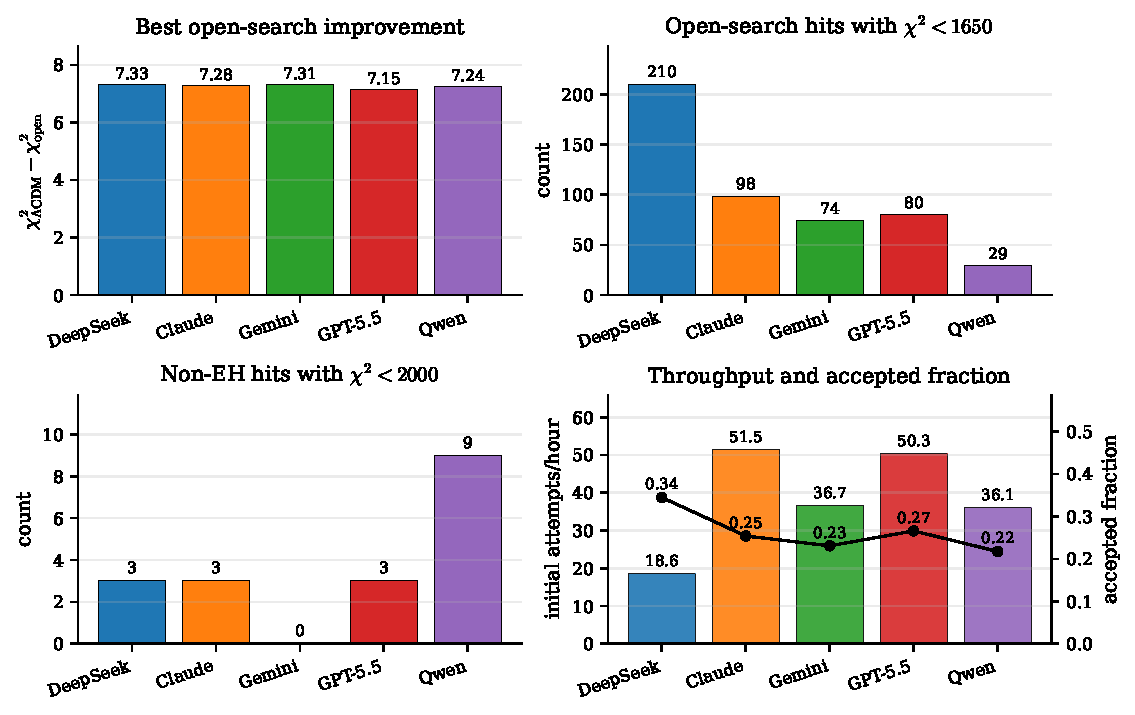
\includegraphics[width=0.88\textwidth]{figures/main_benchmark_dashboard.pdf}
\caption{Summary of the matched five-model benchmark.  Each proposal model received 600 initial theory attempts with the same deterministic validation pipeline.  The panels show the positive open-search improvement $\chi^2_{\Lambda{\rm CDM}}-\chi^2_{\rm open}$ relative to the fixed $\Lambda$CDM reference, the number of high-quality open-search hits, the number of viable non-EH hits with $\chi^2_{\rm tot}<2000$, and the initial-attempt throughput together with the accepted fraction.}
\label{fig:benchmark-dashboard}
\end{figure*}

\begin{table*}[t]
\centering
\caption{Final matched 600-attempt benchmark.  ``Open'' denotes the full grammar sector, while ``non-EH'' denotes the sector without a bare Einstein--Hilbert $R$ anchor.  Rates are computed from all recorded validation attempts, including expanded/refined attempts when present.  The throughput column counts initial attempts per wall-clock hour.}
\label{tab:agent-benchmark}
\resizebox{\textwidth}{!}{%
\begin{tabular}{lcccccccc}
\toprule
Proposal model & Best $\chi^2$ & Open best & Open median & Open $<1650$ & non-EH best & non-EH $<2000$ & Throughput & Accepted rate \\
\midrule
DeepSeek V4 Pro & 1637.953 & 1637.953 & 1637.956 & 210 & 1946.871 & 3 & 18.6 & 0.345 \\
Gemini 3.1 Pro & 1637.969 & 1637.969 & 1638.905 & 74 & 2492.845 & 0 & 36.7 & 0.231 \\
Claude Opus 4.8 & 1637.995 & 1637.995 & 1638.781 & 98 & 1946.871 & 3 & 51.5 & 0.254 \\
Qwen 3.7 Plus & 1638.035 & 1638.035 & 2728.138 & 29 & 1946.871 & 9 & 36.1 & 0.217 \\
GPT-5.5 & 1638.130 & 1638.130 & 1641.321 & 80 & 1946.871 & 3 & 50.3 & 0.266 \\
\bottomrule
\end{tabular}}
\end{table*}

Table~\ref{tab:agent-benchmark} and Fig.~\ref{fig:benchmark-dashboard} show that all five proposal policies find open-search backgrounds improving on the fixed $\Lambda$CDM reference by about seven units in $\chi^2_{\rm tot}$.  The ranking by the single best background is DeepSeek V4 Pro, Gemini 3.1 Pro, Claude Opus 4.8, Qwen 3.7 Plus, and GPT-5.5, but the differences in the best open-search values are small compared with the differences in search behavior.  DeepSeek produces a very dense basin of high-quality open-search hits, with an accepted median essentially at its best value.  Claude and GPT-5.5 are substantially faster and still find competitive optima.  Qwen has the weakest open-search stability, as indicated by its high accepted median, but it produces the largest number of non-EH hits below $\chi^2_{\rm tot}=2000$.  Gemini reaches a strong open-search optimum but does not find a non-EH hit below 2000 in this run.

\begin{figure*}[t]
\centering
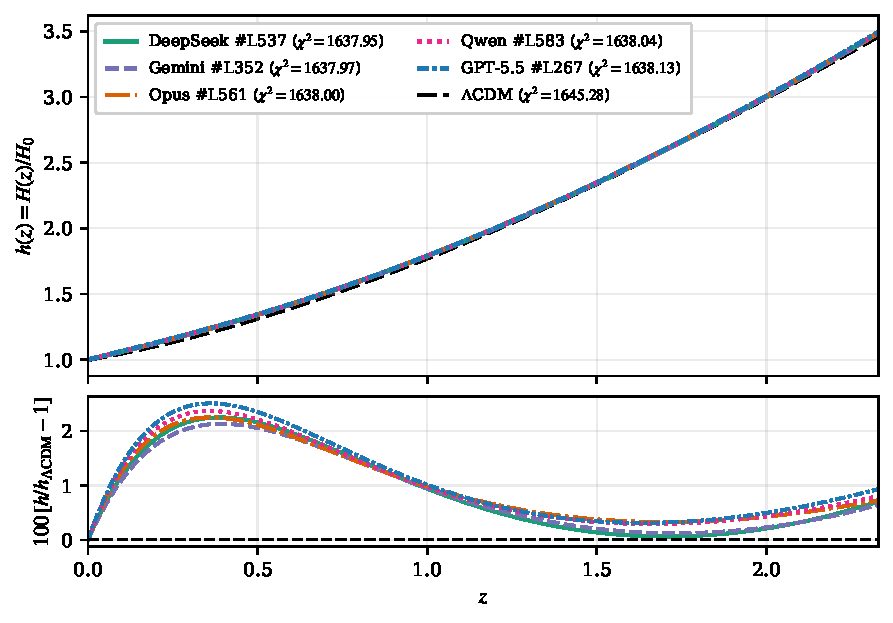
\includegraphics[width=0.88\textwidth]{figures/agent_best_h_lcdm.pdf}
\caption{Expansion histories for the best open-search theory found by each proposal model in the matched 600-attempt benchmark, compared with the fixed $\Lambda$CDM reference.  The labels give the proposal model, the scheduler theory identifier in the old run, and the corresponding total $\chi^2$.  The lower panel shows the percent-level residual relative to the $\Lambda$CDM expansion history.}
\label{fig:agent-best-h-lcdm}
\end{figure*}

\begin{figure*}[t]
\centering
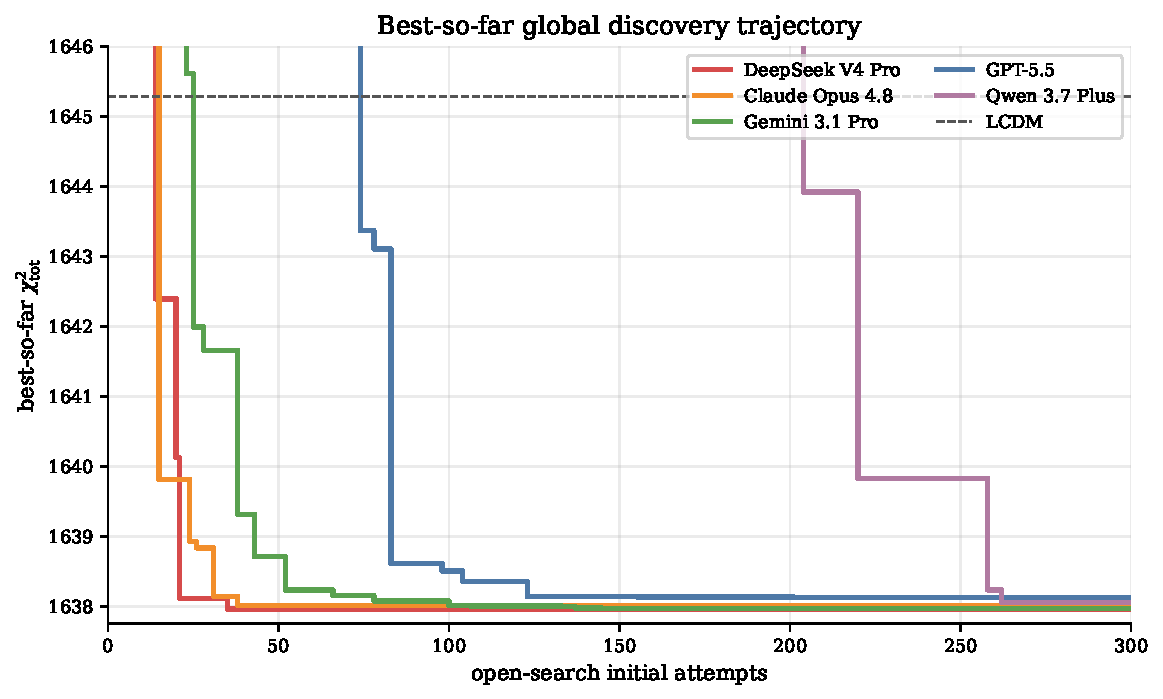
\includegraphics[width=0.88\textwidth]{figures/best_so_far_open_search.pdf}
\caption{Best-so-far open-search trajectory as a function of completed open-search initial attempts.  The dashed line is the fixed $\Lambda$CDM reference.  The figure separates proposal speed in the structural search from the final physical ranking; all curves are evaluated by the same Solver likelihood.}
\label{fig:best-so-far-open}
\end{figure*}

\subsection{Open-search backgrounds}
\label{subsec:open-search-results}

The open-search sector answers whether the proposal policy can find the best background histories allowed by the full grammar.  The robust qualitative result is that the best backgrounds remain Einstein--Hilbert anchored.  Many of them are nearly degenerate with EH plus scalar baselines, but several leading representatives contain explicit curvature corrections that are not numerically negligible according to the effective-size diagnostic.

The following representatives are displayed as coefficient-substituted densities rather than as schematic operator lists.  We retain the fixed scalar matter terms and omit only terms whose fitted coefficients are exactly zero.  Scientific notation is used for compactness.

\begin{widetext}
\begingroup\small
\begin{align}
\mathscr{L}^{\rm open}_{\rm DS}
&=\sqrt{-g}\Bigg\{
\Mp^2\left[
0.5\,R
+2.19455\times10^{16}\,\Lam^{-3}\phi_2
R^a{}_{bcd}R_a{}^{bcd}
\right]
-\frac12 g^{\mu\nu}\nabla_\mu\phi_1\nabla_\nu\phi_1
-m_1^2f_1^2\left[1-\cos\left(\frac{\phi_1}{f_1}\right)\right]
-\frac12 g^{\mu\nu}\nabla_\mu\phi_2\nabla_\nu\phi_2
-\frac12 m_2^2\phi_2^2
\Bigg\},
\nonumber\\[-1mm]
&\hspace{1cm}
\chiT=1637.953,
\qquad
\Delta_{\rm max}=3.91 ,
\label{eq:deepseek-open-model}
\\[1mm]
\mathscr{L}^{\rm open}_{\rm Gemini}
&=\sqrt{-g}\Bigg\{
\Mp^2\left[
0.5\,R
+1.39011\times10^{19}\,\Lam^{-4}\phi_1\phi_2 R^2
\right]
-\frac12 g^{\mu\nu}\nabla_\mu\phi_1\nabla_\nu\phi_1
-\frac12 m_1^2\phi_1^2
-\frac12 g^{\mu\nu}\nabla_\mu\phi_2\nabla_\nu\phi_2
-\frac12 m_2^2\phi_2^2
\Bigg\},
\nonumber\\[-1mm]
&\hspace{1cm}
\chiT=1637.969,
\qquad
\Delta_{\rm max}=1.15\times10^{2} ,
\label{eq:gemini-open-model}
\\[1mm]
\mathscr{L}^{\rm open}_{\rm Claude}
&=\sqrt{-g}\Bigg\{
\Mp^2\left[
0.5\,R
-2.63959\times10^{12}\,\Lam^{-2}R^2
-6.33289\times10^{-10}\,\Lam^{-4}R\,R^{ab}R_{ab}
\right.\nonumber\\
&\hspace{2.8cm}\left.
+2.44705\times10^{-4}\,\Lam^{-4}
R^{cd}{}_{ab}R^{afh}{}_{c}R^{b}{}_{fdh}
+18.9697\,\Lam^{-4}R_{ab}R^{adef}R^{b}{}_{def}
\right]\nonumber\\
&\hspace{1.2cm}
-\frac12 g^{\mu\nu}\nabla_\mu\phi_1\nabla_\nu\phi_1
-m_1^2f_1^2\left[1-\cos\left(\frac{\phi_1}{f_1}\right)\right]
\Bigg\},
\nonumber\\[-1mm]
&\hspace{1cm}
\chiT=1637.995,
\qquad
\Delta_{\rm max}=7.65\times10^{5}.
\label{eq:claude-open-model}
\end{align}
\endgroup
\end{widetext}

The DeepSeek branch, Eq.~\eqref{eq:deepseek-open-model}, is not merely an EH baseline in the report diagnostic: its dominant $\phi_2R^a{}_{bcd}R_a{}^{bcd}$ correction has relative effect $\Delta_{\rm max}\simeq3.91$.  Gemini's best branch, Eq.~\eqref{eq:gemini-open-model}, activates a two-scalar $\phi_1\phi_2R^2$ correction with an even larger reported relative effect.  Claude's representative, Eq.~\eqref{eq:claude-open-model}, is a $\phi_1$-only higher-curvature branch whose nominal best-fit density is dominated by an $R^2$ coefficient.  These examples suggest that the open-search optimum is not tied to a single covariant operator identity.  The background likelihood admits a family of EH-anchored scalar and curvature-corrected histories with very similar $H(z)$.

The large values of $\Delta_{\rm max}$ should not be over-interpreted as a proof of controlled modified gravity.  They are useful discovery diagnostics, but they also flag branches that require a separate EFT-control and perturbation-stability audit.  DeepSeek, Claude, Gemini, and GPT-5.5 all find many accepted backgrounds below $\chi^2_{\rm tot}=1650$, while some best representatives remain EH only or EH dominated.  Therefore a low background $\chi^2$ should be read as evidence for a high-quality EH-anchored dark-energy basin, not yet as evidence for a unique dynamically active higher-curvature theory.

\subsection{Non-EH new-physics search}
\label{subsec:noneh-results}

\begin{figure*}[t]
\centering
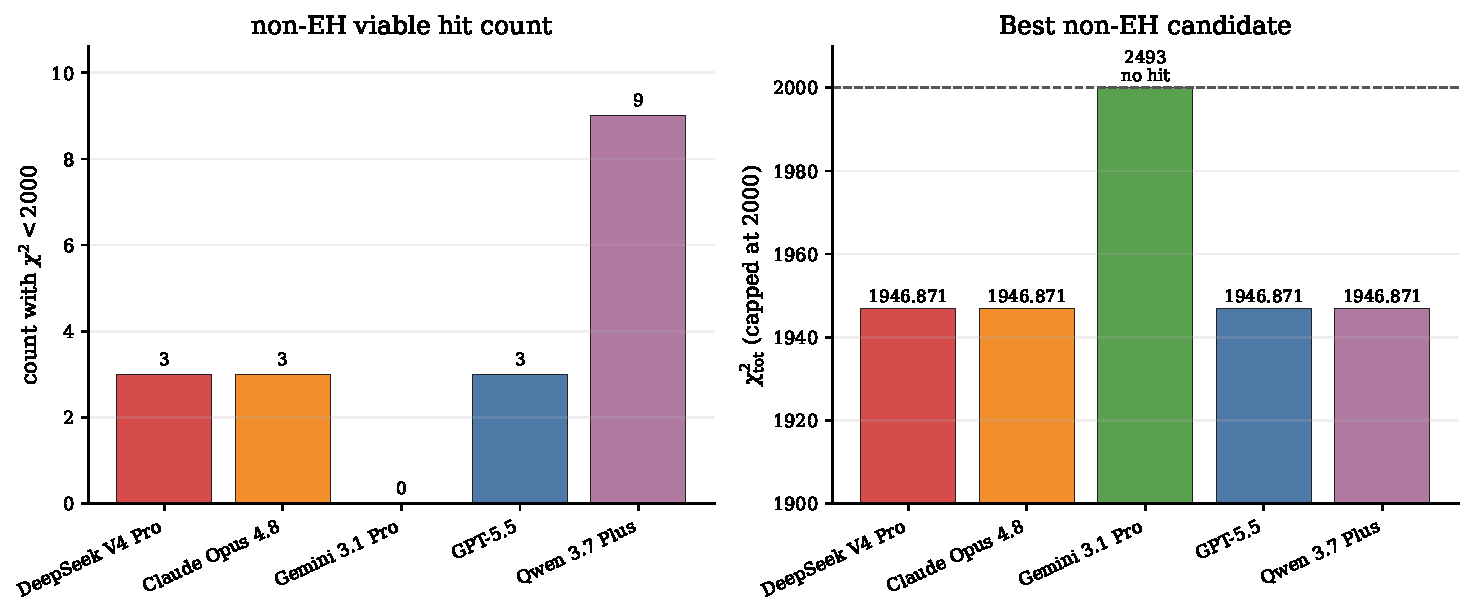
\includegraphics[width=0.88\textwidth]{figures/non_eh_summary.pdf}
\caption{Non-EH search summary.  The left panel counts accepted non-EH families below $\chi^2_{\rm tot}=2000$.  The right panel shows the best non-EH value for each proposal model, capped to the physically relevant range for this sector.  Qwen finds the most viable non-EH hits, while Gemini does not reach the $\chi^2_{\rm tot}<2000$ threshold in this run.}
\label{fig:noneh-summary}
\end{figure*}

The non-EH sector is deliberately harder.  It forbids the bare Einstein--Hilbert $R$ anchor, so a term such as $R^2$ or $\phi_2 R$ may appear, but a standalone EH kinetic term for the metric may not.  This sector is meant to test whether the agent can find genuinely new gravitational backgrounds rather than rediscovering EH plus scalar dark energy.  The resulting fits are much worse than the open-search optima but far from random: four of the five agents repeatedly identify a branch near
\begin{equation}
\chi^2_{\rm tot}\simeq 1946.87 .
\label{eq:noneh-plateau}
\end{equation}
The shared motif is a cutoff-normalized $\phi_2$ sector coupled to Ricci- and Riemann-squared curvature invariants.

The best Qwen representative is slightly lower than the corresponding plateau values from the other agents.  Its coefficient-substituted density is
\begin{widetext}
\begingroup\small
\begin{align}
\mathscr{L}^{\rm non\mbox{-}EH}_{\rm Qwen}
&=\sqrt{-g}\Bigg\{
\Mp^2\left[
1.08514\times10^{-2}\,\Lam^{-4}\phi_2^2 R^{ab}R_{ab}
+6.76759\times10^{10}\,\Lam^{-4}\phi_2^2 R^a{}_{bcd}R_a{}^{bcd}
\right]\nonumber\\
&\hspace{1.2cm}
-7.99776\times10^{15}\,\Lam^{2}\phi_2^2
-67.9540\,\Lam\,\phi_2^3
-1.49225\times10^{-9}\,\Lam^{-2}\phi_2^6
-\frac12 g^{\mu\nu}\nabla_\mu\phi_2\nabla_\nu\phi_2
-m_2^2f_2^2\left[1-\cos\left(\frac{\phi_2}{f_2}\right)\right]
\Bigg\},
\nonumber\\[-1mm]
&\hspace{1cm}
\chiT=1946.870851 .
\label{eq:qwen-noneh-model}
\end{align}
\endgroup
\end{widetext}
OpenAI, Claude, and DeepSeek repeatedly find nearby linear-$\phi_2$ curvature-squared forms.  A compact representative of this common branch is the GPT-5.5 solution
\begin{widetext}
\begingroup\small
\begin{align}
\mathscr{L}^{\rm non\mbox{-}EH}_{\rm GPT}
&=\sqrt{-g}\Bigg\{
\Mp^2\left[
-2443.256\,\Lam^{-3}\phi_2R^{ab}R_{ab}
+2605.845\,\Lam^{-3}\phi_2R^a{}_{bcd}R_a{}^{bcd}
\right]
-\frac12 g^{\mu\nu}\nabla_\mu\phi_2\nabla_\nu\phi_2
-m_2^2f_2^2\left[1-\cos\left(\frac{\phi_2}{f_2}\right)\right]
\Bigg\},
\nonumber\\[-1mm]
&\hspace{1cm}
\chiT=1946.870857 .
\label{eq:gpt-noneh-model}
\end{align}
\endgroup
\end{widetext}
The repeated appearance of Eqs.~\eqref{eq:qwen-noneh-model} and \eqref{eq:gpt-noneh-model} is nontrivial because the agents differ in their proposal distributions and language-model outputs.  It suggests that the current grammar contains a recognizable no-bare-EH FLRW branch driven by $\phi_2$ curvature couplings.

Physically, however, this branch is not competitive with EH-anchored backgrounds.  Its best $\chi^2_{\rm tot}$ is worse than the $\Lambda$CDM reference by about 300 and worse than the best open-search candidates by about 309.  It is therefore not a viable replacement for the EH-anchored dark-energy basin at the background-likelihood level.  Its value is diagnostic: it shows that the search can discover a repeated, runnable, non-EH modified-gravity structure rather than only pathological failures, but it also quantifies how much harder it is for that sector to reproduce late-time distances.

\begin{figure*}[t]
\centering
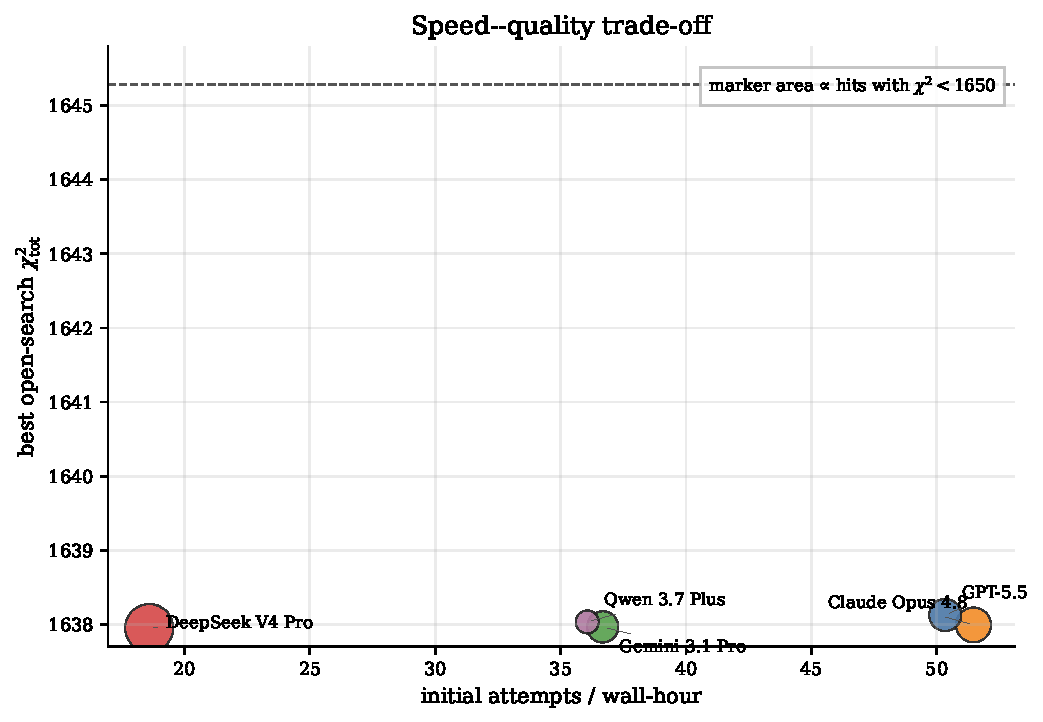
\includegraphics[width=0.88\textwidth]{figures/speed_quality_tradeoff.pdf}
\caption{Speed-quality trade-off.  The horizontal axis gives initial attempts per wall-clock hour and the vertical axis gives the best open-search $\chi^2_{\rm tot}$.  Marker area scales with the number of open-search hits below $\chi^2_{\rm tot}=1650$.  DeepSeek finds the best and most stable open-search basin but is slow; Claude and GPT-5.5 provide the best speed-efficiency compromise.}
\label{fig:speed-quality}
\end{figure*}

\subsection{Agent-level comparison}
\label{subsec:agent-comparison}

The benchmark separates four kinds of performance.  Global optimization is best measured by the minimum $\chi^2_{\rm tot}$ and the best-so-far trajectory in Fig.~\ref{fig:best-so-far-open}.  On this axis DeepSeek, Gemini, Claude, Qwen, and GPT-5.5 all reach the same narrow EH-anchored basin, with DeepSeek slightly ahead in the final best value.  New-physics search is better measured in the non-EH sector: Qwen finds nine non-EH hits below 2000, while OpenAI, Claude, and DeepSeek each find three and Gemini finds none.  Speed/efficiency is captured by initial attempts per wall-hour: Claude and GPT-5.5 run near $50$ attempts/hour, Gemini and Qwen near $36$ attempts/hour, and DeepSeek near $19$ attempts/hour.  Robustness and stability are reflected in acceptance rates and accepted medians: DeepSeek has the strongest open-search acceptance and accepted-median stability, whereas Qwen's high non-EH acceptance comes with a less stable open-search distribution.

The acceptance rate deserves separate attention because it is not the same as scientific quality.  A high acceptance rate means the proposal policy often reaches a Solver-evaluable background, which is useful for learning and throughput.  It does not guarantee a low $\chi^2$ or a physically active correction.  Conversely, a lower acceptance rate can still be acceptable if the surviving candidates are diverse or if the sector is intentionally difficult.  For this reason we treat acceptance rate as a robustness metric, not as the primary ranking metric.

\section{Validation Boundaries and Physical Interpretation}
\label{sec:validation-boundaries}

The validation performed here is a background-level filter, not a complete proof of covariant viability.  The symbolic stage removes independent higher-time derivatives in the homogeneous FLRW equations and the Solver enforces regular integration, the modified Friedmann constraint, and the data likelihood.  A fully viable theory must still pass perturbation-level tests: after solving nondynamical constraints, the scalar and tensor quadratic actions must have positive kinetic eigenvalues, acceptable sound speeds, no rapid gradient instabilities, and a regular constraint structure.  The present DES-SN plus DESI-DR2 BAO likelihood also does not include structure growth, weak lensing, redshift-space distortions, gravitational-wave propagation, or local-gravity screening.

The EFT interpretation is likewise diagnostic rather than automatic.  The trajectory-level cut controls $|H|/\Lambda$, but broad coefficient and scalar priors can still produce branches whose fitted corrections are large compared with the EH term.  We therefore report the effective correction size $\Delta_{\rm max}$ for EH-anchored representatives.  Small values indicate an EH-dominated fit; values of order unity or larger identify branches that may contain active modified gravity but require a follow-up hierarchy audit involving scalar amplitudes, scalar kinetic scales, and adjacent-operator ratios.  Finally, accepted operator lists need not be inequivalent covariant theories: integration by parts, field redefinitions, curvature identities, and FLRW degeneracies can map different raw operator lists to the same background equations.  The results should therefore be read as best-per-family background representatives, pending a full operator-basis and perturbation audit.



\section{Discussion and Conclusions}
\label{sec:conclusion}

The final benchmark demonstrates that the deterministic modified-gravity pipeline can be used not only to search for backgrounds but also to compare proposal agents in a reproducible way.  Because every candidate is passed through the same grammar, FLRW derivative-order filter, Builder, Solver, and DES-SN plus DESI-DR2 likelihood, the differences in Table~\ref{tab:agent-benchmark} primarily reflect differences in proposal behavior rather than differences in downstream physics.

The main physics conclusion is conservative.  The open-search sector consistently rediscovers an EH-anchored scalar dark-energy basin with $\chi^2_{\rm tot}\simeq1638$, about seven units below the fixed $\Lambda$CDM reference used here.  Some representatives in this basin contain active curvature corrections, including $\phi_2R_{\mu\nu\rho\sigma}R^{\mu\nu\rho\sigma}$ and $\phi_1\phi_2R^2$, but many nearly degenerate representatives are EH only or EH dominated.  Background data alone therefore cannot determine whether the improvement should be interpreted as evidence for a dynamically important higher-curvature correction.  It identifies candidate branches for follow-up.

The non-EH search gives a complementary result.  Several agents independently find a $\phi_2$ curvature-coupled branch near $\chi^2_{\rm tot}=1946.87$.  This is an interesting new-physics structure because it is runnable, repeated, and substantially better than the generic non-EH failure plateau near $\chi^2_{\rm tot}\simeq9434$.  It is nevertheless far worse than both $\Lambda$CDM and the EH-anchored open-search basin.  In the current grammar and priors, the non-EH branch is therefore a useful diagnostic target rather than a viable late-time background replacement.

At the agent level, the best proposal policy depends on the objective.  DeepSeek V4 Pro gives the best and most stable open-search basin but at the highest wall-clock cost.  Claude Opus 4.8 and GPT-5.5 provide the best speed-quality compromise.  Qwen 3.7 Plus is the strongest new-physics explorer by non-EH hit count, despite weaker open-search stability.  Gemini 3.1 Pro reaches a strong global optimum but underperforms in the non-EH sector in this run.  This separation of objectives is important for future studies: a single scalar leaderboard hides the difference between global background optimization and deliberate exploration of difficult non-EH theory classes.

Future work should add perturbation-level stability, growth and lensing likelihoods, gravitational-wave propagation constraints, local-gravity screening checks, and an operator-basis audit that removes FLRW-equivalent representatives.  Longer non-EH runs with targeted priors may clarify whether the $\phi_2$ curvature branch can be improved or whether the absence of a bare EH anchor is fundamentally disfavored by the background data.  The same benchmark protocol can also be extended to additional proposal models, with cost and latency recorded alongside physics metrics.

\bibliographystyle{apsrev4-2}
\bibliography{main2}

\end{document}
